\graphicspath{ {figures/metabolism/} }

% CONTRIBUTIONS
%%%%%%%%%%%%%%%%%%%%%%%%%%%%%%%%%%%

\chapter{Repressive gene regulation synchronizes development with cellular metabolism}
\label{ch:metabolism}

A manuscript closely resembling this chapter was coauthored with Justin Cassidy, Rachael Bakker, Ritika Giri, Nicol\'{a}s Pel\'{a}ez, Bryan Eder, Anna Bobrowska, Neda Bagheri, Lu\'{i}s Amaral, and Richard Carthew. A preprint is publicly available at \url{https://doi.org/10.1101/548032}. 

All of the experiments detailed in this chapter were conceived, designed, and executed by my colleagues. In particular, Justin Cassidy obtained the wealth of data that ultimately made this work possible. My personal contributions include all of the computational modeling and simulations. All of the text included in this chapter was either written by or under the guidance of Professor Richard Carthew, whose lab conducted all of the experiments.

% MANUSCRIPT
%%%%%%%%%%%%%%%%%%%%%%%%%%%%%%%%%%%% 

\section{Introduction}

Animal development occurs over a defined timescale, which requires control of the rates of developmental processes. Developmental timescales are an intrinsic feature of a species, and are not necessarily determined by external clocks \cite{Ebisuya2018}. Rather, the pace of development is encoded in the genome. Development occurs via a stereotypic sequence of events involving cell division, growth, movement, apoptosis, polarization, and differentiation. Correct assembly of functional structures depends upon synchronization of cell division and differentiation events \cite{Foe1989,Sulston1983}. Small variation in timing produces variation in structure that is observed between individuals \cite{Francesconi2014,Poullet2016}. Abnormal timing can result in structural defects that lead to compromised survival \cite{Moss2007}.

While developmental tempo is a fundamental property of a species, it can vary under different conditions. For example, temperature affects the pace of development in many ectotherms, such as arthropods, nematodes, fish, and reptiles \cite{Atlas1935,Davidson1944,Kuntz2014,Zuo2011}. Diet and food intake also affect organismal growth rate and the pace of development for many species, including humans \cite{Arendt1997,Brown2004,Metcalfe2001,Pontzer2016}. Finally, cellular metabolism can alter the pace of development. For example, the evolutionarily conserved \textit{Clk1} gene encodes a mitochondrial enzyme necessary for normal cellular respiration \cite{Felkai1999}, and loss of the \textit{clk1} gene in nematodes and mice results in developmental delays \cite{Levavasseur2001,Nakai2001,Wong1995}. In \textit{Drosophila}, restricting glucose consumption by cells slows development \cite{Brogiolo2001,Layalle2008,Rulifson2002,Shingleton2005}. West and colleagues formulated a general quantitative model that relates developmental tempo to both cellular metabolic rate and temperature \cite{Gillooly2002}. Strikingly, the model fits meta-data spanning several kingdoms, suggesting a universal relationship between metabolism and developmental tempo.

Many developmental processes involve specification of different cell types in a stereotyped sequence. All of these differentiated cell types originate from progenitor cells. The sequence of cell differentiation is driven by changes in the gene expression program within progenitors. Gene regulators, typically transcription factors, are sequentially activated and repressed, resulting in transient periods of increased activity. During these periods, they change gene expression in the progenitors. This coincides with and causes a temporal series of cell fate decisions. Since these regulators frequently interact with one another, the entire cascade constitutes a gene regulatory network (GRN). Such GRNs have been characterized for embryogenesis \cite{Cusanovich2018,Lawrence1992}, development of the central nervous system \cite{Kohwi2013}, and development of the sensory nervous system \cite{Cepko2014}. Because the tempo of development can vary, GRN dynamics must be able to reliably adjust to a variable timing mechanism. Therefore, understanding how these GRNs adapt to a variable timescale is crucial for understanding the mechanisms of animal development.

Phenomenological observations suggest that there are limits to the timescales to which development may adapt. While broiler chickens have been successfully bred for rapid growth, frequent abnormalities in musculoskeletal development are evident in such breeds \cite{Julian2005,Whitehead2003}. Animals (and humans) experience hyper-normal growth rates if they initially experience delayed growth \cite{Arendt1997}. Such compensatory growth is linked to a variety of developmental and physiological defects \cite{Metcalfe2001}. Conversely, slowing growth can alleviate defects caused by mutations that impair development. As first noted by T.H. Morgan, morphological phenotypes can be suppressed by limiting the nutrition of mutant animals \cite{Child1939,Morgan1915,Morgan1929,Sang1963}. Likewise, raising animals under lowered temperatures can sometimes suppress the phenotypes of mutations that are not classical \textit{ts} alleles \cite{Child1935,Krafka1920,Lewis1980,Villee1943}. Collectively, these observations suggest an unknown mechanism ensures successful developmental outcomes amidst variability in developmental tempo.

Here, we have explored this mechanism. We find that impairing gene repression in GRNs causes developmental errors but only when cell metabolism and growth rate are normal. When either energy metabolism or protein anabolism are reduced, developmental errors are reduced or even suppressed. We find that this relationship between metabolism and repression is so prevalent that the entire microRNA family becomes unnecessary when metabolism is slowed. Using a general quantitative modeling framework for regulated gene expression, we show that multiple layers of weak repression render gene expression dynamics independent of variable biochemical rates. When rates are modestly reduced, fewer repressors are needed to ensure normal expression dynamics. We experimentally validate this model prediction by following GRN dynamics in \textit{Drosophila}. Our findings support a new mechanism whereby layers of gene repression allow development to occur over a wider range of time scales, enabling development to proceed faster if metabolic conditions allow for it. The need for flexible error frequency suppression could provide an evolutionary impetus for the high prevalence of genetic redundancy.

\section{Results}

Developmental patterns arise from directed dynamics of cell-cell signaling and gene regulation. The sensory organs of \textit{Drosophila} are a classic system with which to study these phenomena \cite{Quan2005}. A broad collection of gene mutations has specific effects on the formation of various sensory organs, and these mutations have been instrumental in uncovering the molecular mechanisms of sensory organ development. The affected genes encode transcription factors, microRNAs, signaling factors, and other gene regulators. We used such gene mutations to readdress the relationship between reduced metabolism and phenotype suppression that was first observed by Morgan \cite{Morgan1915,Morgan1929}. We did so by scoring \textit{Drosophila} sensory mutant phenotypes under conditions of reduced energy metabolism. We generated animals that had reduced metabolism by genetic ablation of their insulin producing cells (IPCs) in the brain (Fig. \ref{fig:metabolism:fig1a}A). This ablation reduces the amount of glucose that cells consume \cite{Rulifson2002}, resulting in 70\% slower development (Fig. \ref{fig:metabolism:fig1a}B), and small but normally proportioned adults (Fig. \ref{fig:metabolism:fig1a}C) \cite{Rulifson2002}.

\begin{figure}[h!]
\label{fig:metabolism:fig1a}
\centering
\includegraphics[scale=1.0]{./figure_1a}
\caption[IPC ablation slows development by restricting energy metabolism.]{\textbf{IPC ablation slows development by restricting energy metabolism.} (A) Strategy to ablate IPCs (red) in the young fly brain. Gal4 expressed under control of the promoter for the \textit{Insulin-Like Peptide 2} (\textit{ILP2}) gene drives production of the pro-apoptotic protein Reaper (Rpr) specifically in IPCs of the brain. (B) The number of days after egg laying (AEL) at which the first individual in either wildtype or $ILP2>Rpr$ populations eclosed (hatched from pupa into adult) is shown, as is the time at which the last individual in each population eclosed. Population sizes for wildtype and $ILP2>Rpr$ were 126 and 185, respectively. (C) Adult body size is affected by IPC ablation. Two females that were raised at the same time and temperature. The left $y w$ animal has normal metabolism, whereas the right animal has slowed metabolism due to ablation of its IPCs.}
\end{figure}

\section{Mutation of repressors has less impact when metabolism is reduced}

We first examined mutations affecting formation of the compound eye. The microRNA miR-7 represses expression of the Yan transcription factor in the developing eye \cite{Li2005}. Yan protein is transiently expressed in the eye \cite{Pelaez2015a}, and is cleared from differentiating photoreceptor (R) cells by multiple repressors acting on its transcription, mRNA stability, and protein stability \cite{Graham2010}. When the \textit{miR-7} gene was specifically ablated in the compound eye of an otherwise wildtype animal, it resulted in small malformed adult eyes due to errors in R cell differentiation (Fig. \ref{fig:metabolism:fig1b}A). This phenotype was highly penetrant in genetically mosaic animals (Fig. \ref{fig:metabolism:fig1b}B). However, when energy metabolism was slowed by IPC ablation, loss of \textit{miR-7} was much less important for the formation of correctly patterned eyes (Fig. \ref{fig:metabolism:fig1b}B). We also examined mutations affecting cell-cell signaling. The Sevenless (Sev) receptor tyrosine kinase hyper-activates MAP kinase in certain eye progenitor cells, leading to enhanced turnover of the Yan protein \cite{Rebay1995}. This enables cells to differentiate into R7 photoreceptors \cite{Voas2004}. When \textit{sev} is mutated, cells completely fail to differentiate as R7 photoreceptors. This effect was readily apparent by staining for an R7-specific marker protein (Fig. \ref{fig:metabolism:fig1b}C). However, slowing metabolism allowed a small but significant number of \textit{sev} mutant cells to become R7 photoreceptors (Fig. \ref{fig:metabolism:fig1b}D). Importantly, since the \textit{sev} mutant makes no protein products \cite{Banerjee1987}, rescue of the mutant phenotype was not simply due to more functional Sev protein molecules being present in slowly metabolizing cells.

\begin{figure}[h!]
\label{fig:metabolism:fig1b}
\centering
\includegraphics[scale=1.0]{./figure_1b}
\caption[Eye developmental defects are rescued by slower energy metabolism.]{\textbf{Eye developmental defects are rescued by slower energy metabolism.} (A) Genetically mosaic individuals with a $miR-7^+$ body and a $miR-7$ mutant eye. Left individual with mispatterned eye has its IPCs intact while the right individual with a normally patterned eye has had its IPCs ablated by $ILP2>Rpr$. (B) Eye patterning is more normal if mosaic individuals slowly metabolize due to IPC ablation. Sample population sizes were between 264 and 467 individuals. P values from Chi-square test with Yates\' correction. (C) Eye cells stained for specific protein markers such that R7 cells (white) can be distinguished from other R cells (purple) and bristle cells (green). Each ring-like cluster of R cells is an ommatidium. Null mutation of \textit{sev} results in no R7 cells (right). (D) Slow metabolism due to IPC ablation increases the fraction of ommatidia that contain an R7 cell in \textit{sev} mutants. Each data point represents one eye sample; between 481 and 837 ommatidia were scored for R7 cells within each eye sample. P value is from a one-way ANOVA with Bonferroni correction.}
\end{figure}

We also examined formation of other sensory organs for evidence of metabolic interactions. Large sensory bristles develop in a highly stereotypic pattern over the \textit{Drosophila} body. The protein Senseless (Sens) transiently appears in a cluster of proneural cells before one cell is chosen to differentiate into a sensory bristle \cite{JafarNejad2003}. MicroRNA miR-9a represses Sens protein expression, and \textit{miR-9a} mutants frequently develop ectopic sensory bristles because this repression is missing (Fig. \ref{fig:metabolism:fig2}A,B) \cite{Cassidy2013,Li2006}. However, when \textit{miR-9a} mutants had their IPCs ablated, errors in bristle number were greatly reduced (Fig. \ref{fig:metabolism:fig2}C).

The protein Hairy directly represses transcription of the proneural genes \textit{achaete} and \textit{scute} during selection of cells for bristle fates \cite{Van1994}. Mutation of \textit{hairy} causes some individuals to develop ectopic large bristles. However, this effect of \textit{hairy} mutation was strongly suppressed when energy metabolism was slowed (Fig. \ref{fig:metabolism:fig2}C). We saw a similar effect on a \textit{cis}-regulatory module (CRM) that represses gene transcription. The \textit{Sternopleural} (\textit{Sp-1}) mutation is present in a CRM located on the 3' side of the \textit{wingless} (\textit{wg}) gene \cite{Neumann1996}, causing Wg misexpression and development of ectopic bristles \cite{Neumann1996}. However, the ectopic bristle phenotype of the $wg^{Sp-1}$ mutant was completely reversed under conditions of slowed energy metabolism (Fig. \ref{fig:metabolism:fig2}D).

\begin{figure}[h!]
\label{fig:metabolism:fig2}
\centering
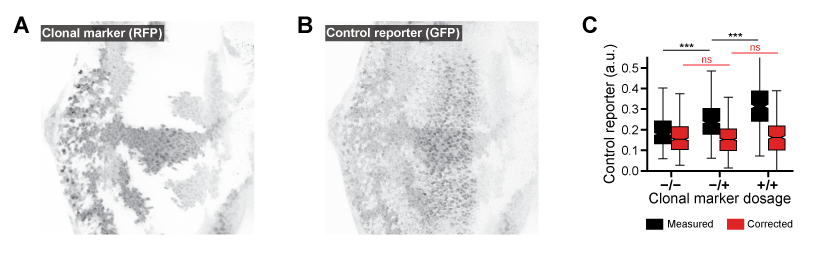
\includegraphics[scale=1.0]{./figure_2}
\caption[Sensory bristle developmental defects are rescued by slower energy metabolism.]{\textbf{Sensory bristle developmental defects are rescued by slower energy metabolism.} (A) Number of scutellar bristles is frequently greater than four in a \textit{miR-9a} mutant whereas it is almost invariably four in wildtype. (B) Distribution of scutellar bristle numbers in wildtype and $miR-9a$ mutant populations. Population sizes for wildtype and $miR-9a$ were 301 and 222, respectively. The cumulative frequency distributions between wildtype and mutant were significantly different ($p<0.0001$, KS test). (C) IPC ablation increases the proportion of $miR-9a$ mutants and \textit{hairy} mutants that have the wildtype number of scutellar bristles. ****, $p<0.0001$; n.s., $p>0.05$ (D) Under normal metabolic conditions, $wg^{Sp-1}$ displays an increased number of sternopleural bristles. IPC ablation dramatically increases the number of mutant individuals with the wildtype number of three sternopleural bristles. Shown in each panel is the number of individuals with bristle number of three versus the total number of individuals scored. IPC ablation significant suppresses the $wg^{Sp-1}$ mutant phenotype ($p<0.0001$, Fishers exact test).}
\end{figure}

\section{MicroRNAs are dispensable when metabolism is reduced}

The mutations thus far examined affect diverse types of regulators, including microRNAs, transcription factors, and signaling molecules. Despite this diversity, all of the mutations have something in common: they affect repressive interactions between genes. To explore the prevalence of this relationship between gene repression and metabolism, we eliminated an entire family of regulatory repressors that control all stages of \textit{Drosophila} development. The microRNA family is composed of 466 distinct microRNAs in \textit{Drosophila melanogaster} \cite{Kozomara2014}. Virtually all microRNAs require Dicer-1 (Dcr-1) protein for their proper biosynthesis, and Ago1 protein as a partner to repress target gene expression \cite{Carthew2009}. Protein-null mutations in either \textit{dcr-1} or \textit{ago1} genes are lethal \cite{Pressman2012}. We raised different null \textit{dcr-1} mutants under conditions of slower energy metabolism, and found that many more animals survived development (Fig. \ref{fig:metabolism:fig3}A). \textit{Ago1} null mutants are normally 100\% embryonic lethal, but mutant lethality was broadly suppressed when animals slowly metabolize due to IPC ablation (Fig. \ref{fig:metabolism:fig3}B). The mutants survived to adulthood, and most survivors had normal eye and bristle patterns as well as other body structures, indicating the rescue of a massive array of developmental defects (Fig. \ref{fig:metabolism:fig3}C). Rescue could also be seen when Ago1 was specifically ablated in cells of the compound eye; eye development was strongly rescued by slower energy metabolism (Fig. \ref{fig:metabolism:fig3}D). Therefore, a major class of regulatory repressors is rendered non-essential when energy metabolism is slowed.

\begin{figure}[h!]
\label{fig:metabolism:fig3}
\centering
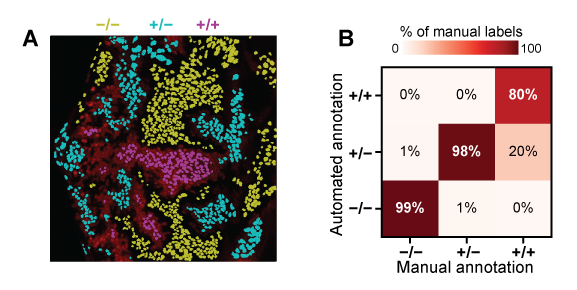
\includegraphics[scale=1.0]{./figure_3}
\caption[The microRNA family is dispensable when energy metabolism is slowed.]{\textbf{The microRNA family is dispensable when energy metabolism is slowed.} (A) The pupal viability of various \textit{dcr-1} nonsense mutants is fully rescued when IPCs are ablated in the mutants. (B) Adult viability of various \textit{ago1} missense and nonsense mutants is rescued when IPCs are ablated in the mutants. (C) Representative \textit{ago1} adults with normal or slowed metabolism. (D) Genetically mosaic individuals with $ago1^+$ bodies and $ago1^{W894X}$ mutant eyes. Left, representative individual with normal metabolism has almost no eye tissue (24/24 animals had this phenotype). Right, representative individual with slowed metabolism has rescued eye tissue. Of 70 such animals analyzed, 46 had this phenotype, 20 had normal eyes, and 4 had eyes that resembled the left animal. This is a statistically significant difference ($p<0.0001$; Chi square with Yates\' correction). Error bars, s.d. ****, $p<0.0001$; **, $p<0.01$; *, $p<0.05$; n.s., $p>0.05$}
\end{figure}

\section{A quantitative model describes the relationship between metabolism and developmental error frequency after repressor loss}

We turned to computational modeling in order to elucidate the biochemical mechanism linking gene repression and metabolism. Because this relationship appears to apply to many GRNs operating at many stages of \textit{Drosophila} development, we sought to model a general feature of dynamical systems rather than the specific regulatory mechanisms behind each of our experimental observations. We therefore explored the mechanism using a general modeling framework for GRNs premised on the progressive restriction of cell potential over time. Each step of restriction corresponds to a change in gene expression (Fig. \ref{fig:metabolism:fig4a}A). A common property of such dynamics is that they are transient; gene products are synthesized, act, and then are eliminated until they are again needed in other cells. This property allows signaling molecules and transcription factors to be repeatedly used to build different body structures at different times.

GRNs use layers of negative regulation to attenuate expression of target genes (Fig. \ref{fig:metabolism:fig4a}B). When these targets are induced by exogenous stimuli, their timely attenuation ensures that protein expression remains transient. The resultant dynamics resemble a simple pulse response, and for this reason classical control theory provides a natural modeling framework (Figs. \ref{fig:metabolism:fig4a}C and \ref{fig:metabolism:figS1a}). In our model, a system of cellular components monitors the relative abundance of a regulatory protein that dictates a cell fate transition. The particular components responsible for implementing control may remain unspecified. Our modeling framework therefore eschews molecular events in favor of minimizing complexity and preserving universality, but preserves the salient features of a detailed molecular mechanism and promotes quantitative predictions.

\begin{figure}[h!]
\label{fig:metabolism:fig4a}
\centering
\includegraphics[scale=1.0]{./figure_4a}
\caption[Modeling gene regulation during cell fate determination.]{\textbf{Modeling gene regulation during cell fate determination.} (A) A program of gene expression occurs as a single cell passes through a series of developmental states. The model focuses on transient expression of a single gene within a cascade of gene expression. A state change is defined as the induction of gene expression by upstream gene products (input) and the action of the gene product (output). (B) Schematic representation of the response to a transient input, which can be either an extracellular or intracellular signal. Gene expression output is subject to layers of negative regulation acting at the gene, transcript, and protein levels. (C) Control representation of a single feedback loop as depicted in B. Boxes contain transfer functions, open circles indicate summation points, and closed circles indicate exclusive switches for each repressor. (D) Protein expression may be subject to layers multiple repressors acting in parallel.}
\end{figure}

A stimulus (the input) activates synthesis of the regulatory protein (the output). Acting in parallel, one or more feedback control elements sense the increase in protein levels and act to down-regulate it, either at the level of gene transcription, mRNA stability, or protein stability. These control elements can be thought of as independent repressors working in parallel to bring the protein level back to a basal steady-state (Fig. \ref{fig:metabolism:fig4a}D). Protein expression follows a biphasic trajectory after reception of a transient stimulus (Fig. \ref{fig:metabolism:fig4b}A,B, left panel). If there were no noise or variability, the protein level would be deterministic over time. However, protein dynamics vary because gene expression is noisy \cite{Arias2006}, something that can be captured in the model simulations by incorporating intrinsic noise.

We then devised a scheme to relate protein expression dynamics to the likelihood of a successful developmental outcome. We define success as the ability of a GRN to attenuate protein expression in a timely manner, thus keeping pace with parallel components of the developmental program by triggering subsequent developmental events. We quantified errors in developmental outcome by defining a threshold that the output protein level must cross before a subsequent event can be triggered. Protein levels exceeding the threshold constitute errors in developmental outcome (Fig. \ref{fig:metabolism:fig4b}B, right panel). Notably, such errors become more frequent when one repressor is removed (Fig. \ref{fig:metabolism:fig4b}C). This property is observed over a broad range of parameter values (Fig. \ref{fig:metabolism:figS1b}), regardless of the manner in which repressors act, or the value at which the threshold is established (Fig. \ref{fig:metabolism:figS1c}).

The modeling framework allowed us to ask whether multiple layers of repression are less important for developmental outcome when energy metabolism is reduced. To answer this question, we halved the rate parameters of each ATP-utilizing reaction to reflect conditions of reduced energy metabolism. Although ATP content remains fairly constant in cells facing limited respiration, the fluxes of ATP synthesis and turnover are affected, manifesting in altered ratios of ATP to ADP and free phosphate \cite{Brown1992}. Anabolic processes such as protein synthesis are highly dependent on the ATP/ADP ratio \cite{Atkinson1977}. When we halved ATP-dependent rate parameters and compared model results from full versus partial repression, we observed that error frequency in developmental outcome did not increase when a repressor was lost (Fig. \ref{fig:metabolism:fig4b}D). This insensitivity to loss of a repressor persisted whether repression was transcriptional, post-transcriptional, or post-translational. The effect was observed across a wide range of model parameter values (Fig. \ref{fig:metabolism:figS2a}A,B), irrespective of where the threshold was set (Fig. \ref{fig:metabolism:figS2a}C), and regardless of whether a basal stimulus was present (Fig. \ref{fig:metabolism:figS2a}D). In many cases the effect remained modestly apparent when the stimulus duration was extended to maintain comparable protein levels under conditions of reduced energy metabolism (Fig. \ref{fig:metabolism:figS2a}E). In general, our modeling framework suggests that the frequency of developmental errors is less sensitive to changes in repression when energy metabolism is reduced.

\begin{figure}[h!]
\label{fig:metabolism:fig4b}
\centering
\includegraphics[scale=1.0]{./figure_4b}
\caption[Simulated developmental errors are less frequent when metabolism is reduced.]{\textbf{Simulated developmental errors are less frequent when metabolism is reduced.} (A-C) Simulated emergence of developmental errors. (A) A transient input signal drives (B) pulsatile protein expression dynamics. Simulations may be performed with two post-translational repressors in place (full repression), or with only one repressor in place (partial repression). Shaded regions correspond to the 98\% confidence band of simulated protein trajectories. We define the commitment time as the time needed for 99\% of simulations with full repression to cross a predefined threshold. With partial repression, the protein levels take longer to decay, so fewer simulations cross the threshold within the defined commitment time. We interpret each failure of a simulated protein level to decay below the threshold in time as a developmental error. (C) Error frequency is greater with partial repression. (D) The model suggests that errors will occur more frequently under partial repression regardless of how repressors act on gene expression (left panel). However, partial repression imparts fewer developmental errors when ATP-dependent parameter values are reduced by 50\% (right panel).}
\end{figure}

Our modeling framework for regulated gene expression promotes simplicity at the expense of two notable limitations. First, the number of transcriptionally active sites within a cell is limited by gene copy number, but the activated-DNA state in our initial linear model was unbounded. To test whether error frequency suppression persists when an upper bound on gene activity is introduced, we considered a simple two-state transcription model. Despite the limitation placed on gene activity, error frequencies remained broadly suppressed when ATP-dependent rate parameters were reduced (Fig. \ref{fig:metabolism:figS2a}F).

Second, gene expression models frequently utilize cooperative kinetics in order to reproduce the nonlinearities and thresholds encountered in transcriptional regulation. We captured these dynamics by reformulating our gene expression modeling framework in terms of Hill kinetics. A parameter sweep revealed that despite the incorporation of cooperative kinetics, error frequencies remained elevated under normal conditions and broadly suppressed when ATP-dependent rate parameters are reduced (Fig. \ref{fig:metabolism:figS2a}G).

Reduced glucose consumption by cells might not only limit ATP fluxes, but also hinder the synthesis of nucleotide and amino acid precursors required for RNA and protein synthesis. To simulate this scenario, we specifically reduced the rate parameters for RNA and protein production. Constraining these synthesis rates also suppressed the rise in error frequency when a repressor was lost (Fig. \ref{fig:metabolism:figS2b}).

Overall, our modeling framework is fully consistent with our experimental observations that multiple layers of repression cease to be important for developmental success under conditions of reduced carbon and energy metabolism. Furthermore, the modeling framework suggests that the phenotype suppression phenomenon may be driven by differences in protein expression dynamics that are dependent on metabolic conditions.

\section{Protein expression dynamics after partial repressor loss}

We quantified the extent to which the expression dynamics underlying developmental events were affected in our model. We first constructed a 98\% confidence band around the set of trajectories simulated with the full complement of repressors (Fig. \ref{fig:metabolism:figS3}A). This confidence band provides lower and upper bounds for the expected protein level. We then evaluated the fraction of trajectories simulated with one repressor missing that fell above or below the confidence band at each point in time. Averaging these values across the time course yields a single metric that reflects the extent to which protein dynamics are affected by the loss of a repressor (Fig. \ref{fig:metabolism:figS3}B). We evaluated this metric for a scenario in which an auxiliary post-transcriptional repressor, akin to a microRNA, is lost. Using typical metabolic parameters, 78\% of trajectories simulated without the post-transcriptional repressor exceed the confidence band generated under full repression (Fig. \ref{fig:metabolism:fig5}A). This overexpression effect is highly robust to parameter variation in the model (Fig. \ref{fig:metabolism:figS3}C). When ATP-dependent parameters were halved, only 16\% of trajectories exceeded the confidence band (Fig. \ref{fig:metabolism:fig5}B). The strong diminishment of overexpression under low metabolic conditions was robust to extensive parameter variation (Fig. \ref{fig:metabolism:figS3}D). These results led us to predict that protein expression dynamics would be much less sensitive to repressor loss if we reduced metabolic rate.

We experimentally tested these predictions by measuring the expression dynamics of a key developmental regulatory protein, Yan. As shown in Chapter \ref{ch:ratio}, Yan exhibits pulsatile dynamics in the larval eye disc, where its expression is induced by a morphogenetic furrow that traverses the eye disc. Eye disc cells located in the morphogenetic furrow rapidly upregulate Yan protein abundance, as quantified by a YFP-tagged version \cite{Pelaez2015a}. Yan levels then gradually decay back to initial conditions within these cells, thus exhibiting pulsatile dynamics. We compared Yan-YFP dynamics in eye disc cells from normally metabolizing larvae and larvae with ablated IPCs (Fig. \ref{fig:metabolism:fig5}C,D). The same pulsatile dynamics were observed in both, but the amplitude of the pulse was slightly reduced and the duration was extended when metabolism was slower. Similar trends were predicted \textit{in silico} (Fig. \ref{fig:metabolism:fig5}A,B).

\begin{figure}[h!]
\label{fig:metabolism:fig5}
\centering
\includegraphics[scale=1.0]{./figure_5}
\caption[Expression dynamics are resistant to repressor loss when energy metabolism is reduced.]{\textbf{Expression dynamics are resistant to repressor loss when energy metabolism is reduced.} (A,B) Simulated expression of target protein output when it is under control of an auxiliary post-transcriptional repressor (green) or not under control of the repressor (orange). All simulations (green and orange) are also under control of a constitutive repressor. Shown are ten randomly-chosen samples from a total population of 5000 trajectories for each condition. (A) Simulations performed with normal ATP-dependent reaction rates. (B) Simulations performed following a 50\% reduction in the rate of ATP-dependent reactions. (C,D) Yan-YFP protein dynamics in eye disc progenitor cells. Time 0 marks the time at which Yan-YFP induction occurs. Solid lines are moving line averages. Shaded regions denote 95\% confidence intervals. Each line average is calculated from a composite of measurements of between 4,379 and 6,716 cells. (C) Yan-YFP dynamics for wildtype $Yan-YFP$ and mutant $Yan^{\Delta miR-7}-YFP$ genes under normal metabolic conditions. (D) Yan-YFP dynamics for wildtype and mutant genes when the IPCs have been ablated.}
\end{figure}

In the eye disc, Yan expression is repressed by the microRNA miR-7 \cite{Li2005}. There are four binding sites for miR-7 in the 3'UTR of \textit{yan} mRNA, and their mutation causes de-repression of Yan output. We eliminated miR-7 repression of \textit{Yan-YFP} by mutating the four binding sites in the 3'UTR of \textit{Yan-YFP} mRNA to make $Yan^{\Delta miR-7}-YFP$. In normally metabolizing eye discs, Yan-YFP protein made from the mutated gene pulsed with greater amplitude and showed impaired decay when compared to Yan-YFP made from the wildtype gene (Fig. \ref{fig:metabolism:fig5}C). These dynamics recapitulate the effect of repressor loss predicted by our model (Fig. \ref{fig:metabolism:fig5}A). In contrast, Yan-YFP made from the mutated gene showed similar dynamics to protein made from the wildtype gene when metabolism was slowed (Fig. \ref{fig:metabolism:fig5}D). This behavior clearly resembled the simulated dynamics under conditions of reduced energy metabolism (Fig. \ref{fig:metabolism:fig5}B).

These measurements demonstrate that miR-7 has little to no impact on Yan expression dynamics when metabolism is slowed, and are consistent with the observed suppression of developmental errors when the same repressor is lost in the eye. The breadth of our model predictions further suggests that these effects are generalizable to other genes and repressors.

\section{Effect of full repression loss}

Our modeling framework is consistent with the hypothesis that multiple weak repressors allow GRN dynamics to faithfully couple to variable energy metabolism, with fewer repressors required when metabolic conditions are reduced. We then asked whether repression is needed at all under such conditions. We studied a model with a full complement of negative control elements and compared the results to a scenario in which all control elements were removed (Fig. \ref{fig:metabolism:fig6}A). Error frequencies approached 100\% under normal growth conditions. While expression dynamics were visibly less affected by repressor loss when ATP-dependent parameters were reduced, the error frequency remained very high (Fig. \ref{fig:metabolism:fig6}B). These results suggest that there are limits to the severity of perturbations for which reductions in energy metabolism can compensate, and reducing energy metabolism does not eliminate the need for gene repression altogether.

To test this prediction, we expressed in the eye a \textit{yan} mutant transgene that is insensitive to all known repression of \textit{yan} transcription, mRNA stability and protein stability \cite{Rebay1995}. The $Yan^{ACT}$ mutant adults had severely disrupted compound eye patterning (Fig. \ref{fig:metabolism:fig6}C). This mutant eye phenotype was not suppressed by ablation of the animals' IPC cells. Wildtype \textit{yan} transgenic adults with normal eye patterning were also unaffected by IPC ablation (Fig. \ref{fig:metabolism:fig6}D).

\begin{figure}[h!]
\label{fig:metabolism:fig6}
\centering
\includegraphics[scale=1.0]{./figure_6}
\caption[Reduced energy metabolism cannot compensate for complete loss of repression.]{\textbf{Reduced energy metabolism cannot compensate for complete loss of repression.} (A,B) Simulated expression of protein output both with (purple) and without (grey) any repression of the target gene. Shown are ten randomly chosen samples from a total population of 5000 trajectories for each condition. Error frequencies exceed 99\% irrespective of metabolic conditions. (A) Simulations performed under normal conditions. (B) Simulations performed following a 50\% reduction in the rate of ATP-dependent reactions. (C) Loss of eye tissue in a $yan^{ACT}$ mutant is not suppressed by slower metabolism. Representative individuals were taken from $N>100$ individuals for each condition. (D) Eye patterning in a $yan^{WT}$ control is not affected by slower metabolism. Representative individuals were taken from $N>100$ individuals for each condition.}
\end{figure}

\section{Limiting protein synthesis reduces the need for repressors}

The coupling of developmental dynamics to time can be explored with other aspects of metabolism. In particular, protein synthesis is an important determinant of rates of growth and development \cite{Lempiainen2009}. We used our modeling framework to investigate the impact of a twofold reduction in overall protein synthesis rate on GRN dynamics. The model suggests that expression dynamics are less affected and fewer developmental errors are incurred by loss of a repressor when protein synthesis rates are reduced (Figs. \ref{fig:metabolism:fig7a} and \ref{fig:metabolism:figS4}A-G).

\begin{figure}[h!]
\label{fig:metabolism:fig7a}
\centering
\includegraphics[scale=1.0]{./figure_7a}
\caption[Simulated developmental errors are less frequent when protein synthesis is reduced.]{\textbf{Simulated developmental errors are less frequent when protein synthesis is reduced.} The model predicts increased frequency of error with partial repression regardless of how auxiliary repressors act on gene expression (left panel is copied from \ref{fig:metabolism:fig4b}D). However, partial repression induces fewer errors when protein synthesis-dependent parameter values are reduced by 50\% (right panel).}
\end{figure}

We tested this model prediction by genetically reducing the abundance of cytoribosomes in all cells in \textit{Drosophila}. We made use of loss-of-function mutations in genes encoding various ribosomal proteins (RPs), which cause the ``Minute'' syndrome of dominant, haploinsufficient phenotypes, including slower growth and development \cite{Marygold2007,Sæbøelarssen1998}. Heterozygous \textit{RP} mutants reduce the number of ribosomes per cell by approximately 50\%, and a total of 64 \textit{RP} genes exhibit a Minute syndrome when mutated. We selected a subset of these genes to reduce ribosome number.

We combined heterozygous \textit{RP} mutants with the repressor mutations we had previously studied. In all cases, the \textit{RP} mutants suppressed the developmental phenotypes of mutations in \textit{wg}, \textit{miR-7}, \textit{sev}, \textit{hairy}, and \textit{miR-9a} (Fig. \ref{fig:metabolism:fig7b}). This error frequency suppression was precisely the result predicted by our modeling.

\begin{figure}[h!]
\label{fig:metabolism:fig7b}
\centering
\includegraphics[scale=1.0]{./figure_7b}
\caption[Reducing ribosome number rescues sensory organ development when repressors are lost.]{\textbf{Reducing ribosome number rescues sensory organ development when repressors are lost.} (A) Loss of $miR-7$ does not cause adult eye mispatterning when \textit{RpS3} is heterozygous mutant. (B) \textit{sev} mutants have more R7-positive ommatidia when either \textit{RpS3} or \textit{RpS13} are heterozygous mutant. Each datapoint represents one eye sample, and between 481 and 837 ommatidia were scored for R7 cells within each eye sample. (C) $wg^{Sp1}$ heterozygous individuals that are also heterozygous mutant for different \textit{RpS} genes have sternopleural bristle numbers more similar to wildtype. (D) Developmental accuracy is recovered for both $miR-9a$ and \textit{hairy} mutants that are also heterozygous mutant for \textit{RpS13}. For all panels in B-E, error bars, s.d. ****, $p<0.0001$; ***, $p<0.001$; n.s., $p>0.05$.}
\end{figure}

We also tested whether expression dynamics are affected by repressor loss under limiting translation conditions. The Sens protein is transiently expressed in proneural cells during selection of sensory bristle fates in the imaginal wing disc \cite{Nolo2000}. Bordering the presumptive wing margin, stripes of proneural cells express Sens protein over a spectrum of levels, reflecting heterogeneity in Wg and Notch regulation of its expression \cite{JafarNejad2006,Quan2005}. Moreover, miR-9a weakly represses \textit{sens} expression in these cells \cite{Li2006}. We recombineered a 19 kb \textit{sens} transgene, amino-terminally tagged with superfold GFP (sfGFP), that functionally replaced the endogenous \textit{sens} gene \cite{Cassidy2013,Venken2006}. Quantitative measurement of sfGFP fluorescence in individual proneural cells yielded the expected distribution of \textit{sens} expression (Fig. \ref{fig:metabolism:fig7c}A). We compared this distribution to one derived from individuals expressing a mutated sfGFP-\textit{sens} transgene in which its miR-9a binding sites had been mutated \cite{Cassidy2013}. Mutation of the miR-9a binding sites in \textit{sfGFP-sens} shifted the fluorescence distribution, and resulted in an average 1.45-fold increase in sfGFP-Sens levels (Fig. \ref{fig:metabolism:fig7c}B). We then tested the effects of miR-9a on \textit{sfGFP-sens} expression when the \textit{RpS13} gene was heterozygous mutant. Strikingly, loss of miR-9a regulation had less effect on sfGFP-Sens protein levels when ribosome numbers were reduced (Fig. \ref{fig:metabolism:fig7c}B). This behavior clearly resembled the simulated dynamics under conditions of reduced protein synthesis (Fig. \ref{fig:metabolism:figS4}B).

\begin{figure}[h!]
\label{fig:metabolism:fig7c}
\centering
\includegraphics[scale=1.0]{./figure_7c}
\caption[Reducing ribosome number diminishes \textit{sfGFP-sens} overexpression when miR-9a repression is lost.]{\textbf{Reducing ribosome number diminishes \textit{sfGFP-sens} overexpression when miR-9a repression is lost.} (A) Frequency distribution of sfGFP-Sens protein level in cells bordering the wing margin of white prepupal wing discs. Shown are distributions of cells expressing either wildtype \textit{sfGFP-sens} or \textit{sfGFP-sens} in which miR-9a binding sites have been mutated. Each group represents \textgreater{} 15,000 cells. (B) \textit{sfGFP-sens} overexpression caused by miR-9a binding site mutations in \textit{RpS13} wildtype (green) and heterozygous mutant backgrounds (violet). Left panel shows median fold-change. Right panel shows the shift in the fluorescence distribution of sfGFP-Sens-positive cells as determined by a Mann-Whitney-Wilcoxon test. Error bars denote 95\% confidence intervals. Overexpression is attenuated in the \textit{RpS13} heterozygous mutant background.}
\end{figure}

\section{Discussion}

Growth and development are fueled by metabolism. This means that the tempo of development depends on metabolic rate. Thus, the dynamics of developmental gene expression must faithfully adjust to a variable time scale. We have shown that multi-layered weak repression within GRNs plays an unexpected function in synchronizing gene expression dynamics with the variable pace of the developmental program. Multiple repressors are required for accelerated development when metabolism is high, and they become functionally redundant when metabolism is low. Multiple repressors therefore allow for reliable development across a broader range of metabolic conditions than would otherwise be tolerated.

Our model explains long-standing observations linking nutrient limitation to suppression of mutant phenotypes \cite{Morgan1915,Morgan1929}. Presumably, such mutations cripple regulatory genes acting on developmental GRNs. Our model might also offer an explanation as to why animals that undergo above-normal growth exhibit compromised development \cite{Arendt1997,Metcalfe2001}. Wildtype GRNs might function across a limited range of metabolism, with functionality breaking down when metabolism exceeds that range.

Our varied analyses suggest that this relationship between metabolism and repression is ubiquitous. We found that the entire family of 466 microRNAs in \textit{Drosophila melanogaster} can become functionally dispensable when energy metabolism is slowed. The extensive literature on microRNA function in \textit{Drosophila} implicates them in practically all facets of the fruit fly's life \cite{Bushati2007,Carthew2017}. Various explanations have been provided for why this family of weak repressors has flourished in the animal kingdom, chief among them the idea that they act as buffers for gene expression \cite{Ebert2012}. We now posit that microRNAs also provide broad and flexible coupling of many developmental processes to variable timescales resulting from fluctuations in metabolism.

There is an alternative mechanism to explain phenotype suppression by reduced metabolism. This mechanism relies on a steady-state and not dynamical perspective of gene expression. Genome-wide gene expression patterns could conceivably change with organismal growth rate. This is the case for chemostat-grown yeast cells, where the expression of 27\% of all genes correlates with growth rate \cite{Brauer2008}. Most genes associated with stress response are overexpressed when cells grow at a slow rate \cite{Brauer2008,Lu2009}. Such differential gene expression could globally modulate dynamical processes such as protein folding and turnover, among others, and thereby attenuate phenotypes of genetic mutations. Abundance of molecular chaperones has been found to affect the penetrance of diverse gene mutations in \textit{C. elegans} and \textit{Drosophila} \cite{Casanueva2012,Rutherford1998}. However, these global effects do not explain why gene expression dynamics are conditionally dependent upon mutations in regulatory genes. We found that repression of Yan and Sens dynamics by microRNAs become more redundant when metabolic rates are slowed.

Metabolic rate increases exponentially with temperature as described by the Arrhenius equation \cite{Zuo2011}, resulting in an indirect temperature dependence of developmental tempo \cite{Gillooly2002}. Temperature also directly affects the rates of reactions within developmental GRNs \cite{Zuo2011}, yet developmental outcomes are generally robust to fluctuations in temperature across a limited range. Various molecular mechanisms have been invoked to explain this robustness. These include chaperones that create large protein-folding reservoirs \cite{Jarosz2010,Rutherford1998}, and regulatory circuits within interaction networks \cite{Li2009}. Our model suggests a complementary mechanism for developmental robustness against temperature variation. By coupling gene expression dynamics with metabolism, weak repressors might neutralize the metabolic effects of temperature on developmental tempo. Indeed, loss of miR-9a regulation is less impactful on sensory organ development if the growth temperature is lowered \cite{Cassidy2013}. Likewise, raising animals under lowered temperatures can suppress the phenotypes of mutations that are not classical \textit{ts} alleles \cite{Child1935,Krafka1920,Lewis1980,Villee1943}.

Metabolic conditions drive variation about the intrinsic developmental tempo of each species. We have shown that layered weak repression within GRNs enables these fluctuations to occur without causing developmental errors. Metabolic conditions change in both space and time. Perhaps the selective advantage of a reliable developmental outcome amidst variable environmental conditions is a driving force in the evolution of gene regulatory networks.
